\documentclass[border=0pt]{standalone}
% newcommands.tex

\usepackage{amssymb, latexsym}
\usepackage{bbding} % for checkmark and xsolid
\usepackage{mathtools}

% math
\newcommand{\N}{\mathbb{N}}
\newcommand{\set}[1]{\{#1\}}
\newcommand{\bset}[1]{\big\{#1\big\}}
\newcommand{\ps}{\mathcal{P}} % for powerset
\newcommand{\emptyseq}{\emptyset} % or using <>?
\newcommand{\tuple}[1]{\langle#1\rangle} % or using (#1)?
\newcommand{\btuple}[1]{\big\langle#1\big\rangle}

\newcommand{\post}{\mathit{post}}
\newcommand{\comment}{\mathit{comment}}
\newcommand{\emptypost}{\mathit{empty}}
\newcommand{\acct}{\brown{\mathit{acct}}}

\newcommand{\yes}{\green{\Checkmark}}
\newcommand{\no}{\red{\XSolidBrush}}

\newcommand{\Key}{{\sf Key}}
\newcommand{\Val}{{\sf Val}}

\newcommand{\h}{\mathcal{H}}
%%%%%%%%%%%%%%% system models %%%%%%%%%%%%%%%
\newcommand{\E}{E}
\newcommand{\evar}{\mathit{e}}
\newcommand{\fvar}{\mathit{f}}
\newcommand{\Event}{{\sf Event}}
\newcommand{\REvent}{{\sf REvent}}
\newcommand{\WEvent}{{\sf WEvent}}
\newcommand{\HEvent}{{\sf HEvent}}
\newcommand{\op}{{\sf op}}
\newcommand{\Op}{{\sf Op}}
\newcommand{\opvar}{\mathit{op}}
\newcommand{\readevent}{{\sf R}}
\newcommand{\Read}{{\sf Read}\;}
\newcommand{\writeevent}{{\sf W}}
\newcommand{\Write}{{\sf Write}\;}
\newcommand{\WriteTx}{{\sf WriteTx}}
\newcommand{\W}{{\sf W}}
\newcommand{\R}{{\sf R}}
\newcommand{\T}{T}
%%%%%%%%%%%%%%% system models %%%%%%%%%%%%%%%

%%%%%%%%%%%%%%% axioms %%%%%%%%%%%%%%%
\renewcommand{\ae}{\mathcal{A}}
\newcommand{\axiom}{\Phi}
\newcommand{\rel}[1]{\xrightarrow{#1}}
\newcommand{\comp}{\;;\;}
\newcommand{\po}{{\sf po}}
\newcommand{\so}{\textsc{so}}
\newcommand{\rb}{\textsc{rb}}
\newcommand{\cb}{\textsc{cb}}
\newcommand{\vis}{\textsc{vis}}
\newcommand{\ar}{\textsc{ar}}
\newcommand{\hist}{\text{Hist}}
\newcommand{\intaxiom}{\textsc{Int}}
\newcommand{\extaxiom}{\textsc{Ext}}
\newcommand{\sessionaxiom}{\textsc{Session}}
\newcommand{\prefixaxiom}{\textsc{Prefix}}
\newcommand{\rbaxiom}{\textsc{ReturnBefore}}
\newcommand{\cbaxiom}{\textsc{CommitBefore}}
\newcommand{\conflict}{\bowtie}
\newcommand{\noconflictaxiom}{\textsc{NoConflict}}
\newcommand{\realtimesnapshotaxiom}{\textsc{RealtimeSnapshot}}
%%%%%%%%%%%%%%% axioms %%%%%%%%%%%%%%%

%%%%%%%%%%%%%%% consistency models %%%%%%%%%%%%%%%
\newcommand{\si}{\textsc{SI}}
\newcommand{\ansisi}{\textsc{ANSI-SI}}
\newcommand{\rtsi}{\textsc{RealtimeSI}}
\newcommand{\gsi}{\textsc{GSI}}
\newcommand{\parallelsi}{\textsc{PSI}}
\newcommand{\pcsi}{\textsc{PCSI}}
\newcommand{\strongsi}{\textsc{StrongSI}}
\newcommand{\strongsessionsi}{\textsc{SI}} % StrongSessionSI
\newcommand{\sessionsi}{\textsc{SessionSI}}
\newcommand{\nmsi}{\textsc{NMSI}}
\newcommand{\ser}{\textsc{SER}}
%%%%%%%%%%%%%%% consistency models %%%%%%%%%%%%%%%

%%%%%%%%%%%%%%% pseudo-code %%%%%%%%%%%%%%%
\newcommand{\g}{G}
\newcommand{\inducedgraph}{I}
\newcommand{\eithervar}{\mathit{either}}
\newcommand{\orvar}{\mathit{or}}
\newcommand{\reachability}{\textsc{Reachability}}
\newcommand{\reachabilityvar}{\mathit{reachability}}

\newcommand{\vertex}{\mathsf{Vertex}}
\newcommand{\edges}{\mathsf{Edge}}
\newcommand{\cons}{\mathsf{Cons}}

\newcommand{\vvar}{\mathit{v}}
\newcommand{\precvar}{\mathit{prec}}
\newcommand{\egvar}{\mathit{e}}
\newcommand{\edgevar}{\mathit{edge}}
\newcommand{\cvar}{\mathit{c}}
\newcommand{\consvar}{\mathit{cons}}

\newcommand{\BV}{\mathsf{BV}}
\newcommand{\Clause}{\mathsf{Cl}}
\newcommand{\DV}{\mathsf{DV}}
\newcommand{\formula}{\mathcal{F}}

\newcommand{\fromvar}{\mathit{from}}
\newcommand{\tovar}{\mathit{to}}
\newcommand{\typevar}{\mathit{type}}

\newcommand{\graphA}{\mathit{Dep}}
\newcommand{\graphB}{\mathit{AntiDep}}
\newcommand{\knowninducedgraph}{\mathit{KI}}
%%%%%%%%%%%%%%% pseudo-code %%%%%%%%%%%%%%%

%%%%%%%%%%%%%%% proof %%%%%%%%%%%%%%%
\newcommand{\inv}{\textsc{Inv}\;}
\newcommand{\case}{\textsc{Case}}
\newcommand{\casei}{\case\; I}
\newcommand{\caseii}{\case\; II}
%%%%%%%%%%%%%%% proof %%%%%%%%%%%%%%%

%%%%%%%%%%%%%%% checking %%%%%%%%%%%%%%%
\providecommand{\G}{}
\renewcommand{\G}{\mathcal{G}}
\renewcommand{\H}{\mathcal{H}}

\newcommand{\SO}{\textsf{SO}}
\newcommand{\WR}{\textsf{WR}}
\newcommand{\WW}{\textsf{WW}}
\newcommand{\RW}{\textsf{RW}}
%%%%%%%%%%%%%%% checking %%%%%%%%%%%%%%%

% colors
\newcommand{\red}[1]{\textcolor{red}{#1}}
\newcommand{\green}[1]{\textcolor{green}{#1}}
\newcommand{\blue}[1]{\textcolor{blue}{#1}}
\newcommand{\cyan}[1]{\textcolor{cyan}{#1}}
\newcommand{\brown}[1]{\textcolor{brown}{#1}}
\newcommand{\teal}[1]{\textcolor{teal}{#1}}
\newcommand{\purple}[1]{\textcolor{purple}{#1}}

\newcommand{\cobra}{\textsc{Cobra}}

\newcommand{\keyxvar}{\textcolor{cyan}{\mathit{x}}}
\newcommand{\keyyvar}{\textcolor{brown}{\mathit{y}}}
\pagestyle{empty} % Remove page numbering
\usepackage[left=68pt, right=0pt, top=72pt, bottom=0pt]{geometry}

\begin{document}
	\pgfplotsset{height=140pt, width=200pt}
	% https://tex.stackexchange.com/questions/6388/how-to-scale-a-tikzpicture-to-textwidth
	\makeatletter
	\newsavebox{\measure@tikzpicture}
	\NewEnviron{scaletikzpicturetowidth}[1]{%
		\def\tikz@width{#1}%
		\def\tikzscale{1}\begin{lrbox}{\measure@tikzpicture}%
			\BODY
		\end{lrbox}%
		\pgfmathparse{#1/\wd\measure@tikzpicture}%
		\edef\tikzscale{\pgfmathresult}%
		\BODY
	}
	\makeatother
	
	\begin{minipage}{0.48\textwidth}
		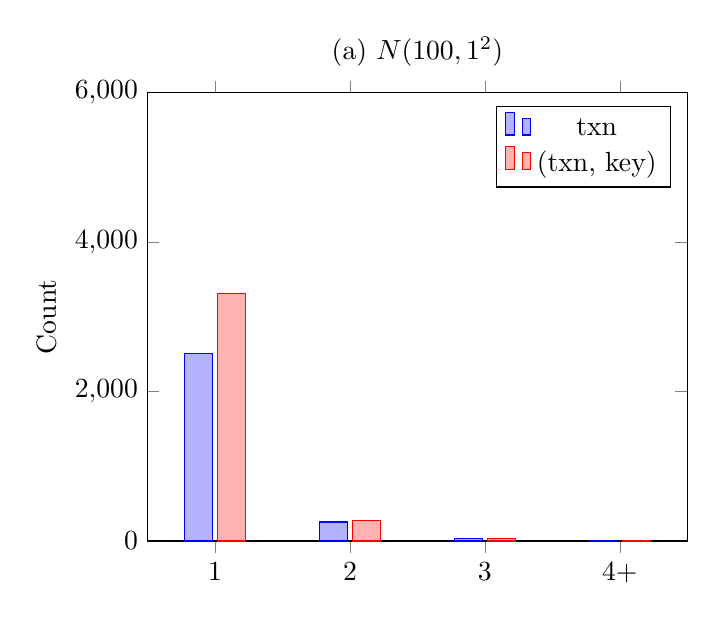
\begin{tikzpicture}
			\begin{axis}[
				x tick label style={draw=none},
				title={(a) $N(100,1^2)$},
				%xlabel={Times},
				ylabel={Count},
				ybar,
				xmin=0.5,
				xmax=4.5,
				ymin=0,
				ymax=6000,
				xtick=data,
				xticklabels={1,2,3,4+},
				legend pos=north east
				]
				\addplot coordinates {(1,2505) (2,255)
					(3,32) (4,8)};
				\addplot coordinates {(1,3317) (2,270) 
					(3,32) (4,8)};
				\legend{txn,(txn, key)}
			\end{axis}
		\end{tikzpicture}
		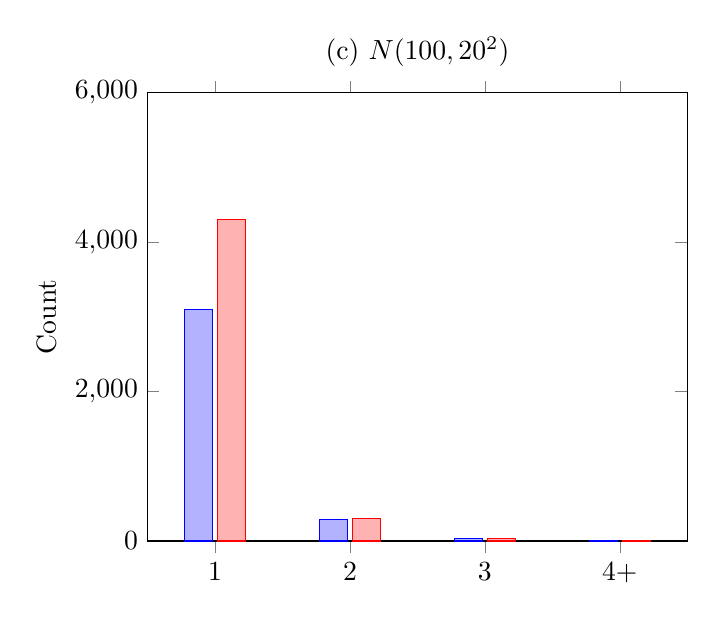
\begin{tikzpicture}
			\begin{axis}[
				x tick label style={draw=none},
				title={(c) $N(100,20^2)$},
				%xlabel={Times},
				ylabel={Count},
				ybar,
				xmin=0.5,
				xmax=4.5,
				ymin=0,
				ymax=6000,
				xtick=data,
				xticklabels={1,2,3,4+},
				legend pos=north east
				]
				\addplot coordinates {(1,3096) (2,285)
					(3,38) (4,3)};
				\addplot coordinates {(1,4307) (2,298) 
					(3,39) (4,3)};
				%\legend{txn,(txn, key)}
			\end{axis}
		\end{tikzpicture}
		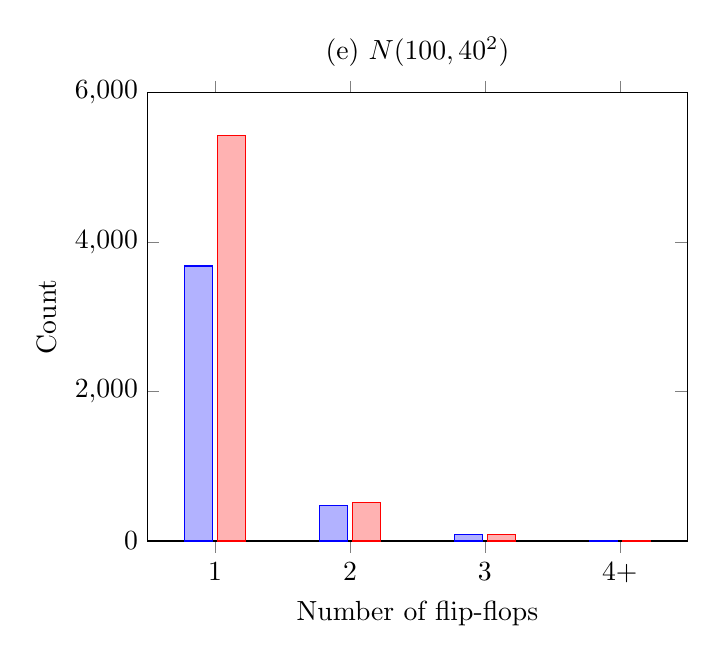
\begin{tikzpicture}
			\begin{axis}[
				x tick label style={draw=none},
				title={(e) $N(100,40^2)$},
				xlabel={Number of flip-flops},
				ylabel={Count},
				ybar,
				xmin=0.5,
				xmax=4.5,
				ymin=0,
				ymax=6000,
				xtick=data,
				xticklabels={1,2,3,4+},
				legend pos=north east
				]
				\addplot coordinates {(1,3681) (2,477)
					(3,86) (4,12)};
				\addplot coordinates {(1,5424) (2,521) 
					(3,88) (4,12)};
				%\legend{txn,(txn, key)}
			\end{axis}
		\end{tikzpicture}
	\end{minipage}
	\hspace{-60pt}
	\begin{minipage}{0.48\textwidth}
		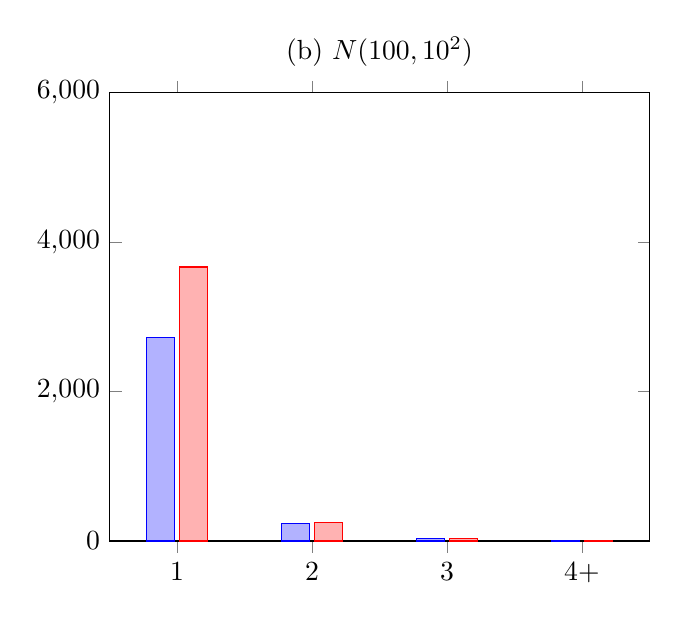
\begin{tikzpicture}
			\begin{axis}[
				x tick label style={draw=none},
				title={(b) $N(100,10^2)$},
				%xlabel={Times},
				%ylabel={Count},
				ybar,
				xmin=0.5,
				xmax=4.5,
				ymin=0,
				ymax=6000,
				xtick=data,
				xticklabels={1,2,3,4+},
				legend pos=north east
				]
				\addplot coordinates {(1,2729) (2,240)
					(3,36) (4,4)};
				\addplot coordinates {(1,3667) (2,247) 
					(3,36) (4,4)};
				%\legend{txn,(txn, key)}
			\end{axis}
		\end{tikzpicture}
		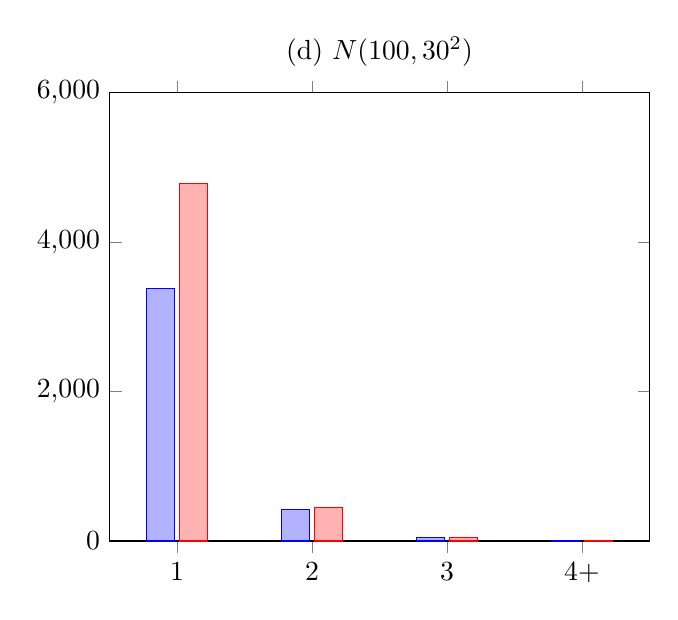
\begin{tikzpicture}
			\begin{axis}[
				x tick label style={draw=none},
				title={(d) $N(100,30^2)$},
				%xlabel={Times},
				%ylabel={Count},
				ybar,
				xmin=0.5,
				xmax=4.5,
				ymin=0,
				ymax=6000,
				xtick=data,
				xticklabels={1,2,3,4+},
				legend pos=north east
				]
				\addplot coordinates {(1,3384) (2,423)
					(3,45) (4,13)};
				\addplot coordinates {(1,4786) (2,447) 
					(3,46) (4,13)};
				%\legend{txn,(txn, key)}
			\end{axis}
		\end{tikzpicture}
		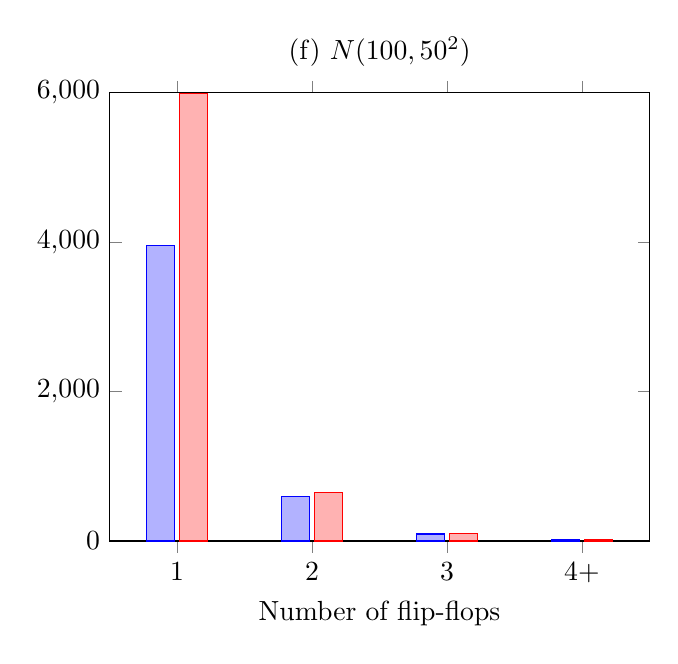
\begin{tikzpicture}
			\begin{axis}[
				x tick label style={draw=none},
				title={(f) $N(100,50^2)$},
				xlabel={Number of flip-flops},
				%ylabel={Count},
				ybar,
				xmin=0.5,
				xmax=4.5,
				ymin=0,
				ymax=6000,
				xtick=data,
				xticklabels={1,2,3,4+},
				legend pos=north east
				]
				\addplot coordinates {(1,3956) (2,600)
					(3,94) (4,21)};
				\addplot coordinates {(1,5990) (2,648) 
					(3,95) (4,21)};
				%\legend{txn,(txn, key)}
			\end{axis}
		\end{tikzpicture}
	\end{minipage}
	\hspace{-80pt}
\end{document}